\subsubsection{Oublions MSVC}

Sous Windows, \ac{SEH} concerne la gestion d'exceptions. Ce mécanisme est indépendant du langage
de programmation et n'est en aucun cas spécifique ni à \Cpp, ni à l'\ac{OOP}.

Nous nous intéressons donc au \ac{SEH} indépendamment du C++ et des extensions du langage dans MSVC.

\myindex{Windows!TIB}
\myindex{Windows!Win32!RaiseException()}

À chaque processus est associé une chaîne de gestionnaires \ac{SEH}. A tout moment, chaque \ac{TIB}
référence le gestionnaire le plus récent de la chaîne.

Dès qu'une exception intervient (division par zéro, violation d'accès mémoire, exception explicitement
déclenchée par le programme en appelant la fonction \TT{RaiseException()} ...), l'OS retrouve dans le
\ac{TIB} le gestionnaire le plus récemment déclaré et l'appelle. Il lui fourni l'état de la \ac{CPU}
(contenu des registres ...) tels qu'ils étaient lors du déclenchement de l'exception.

Le gestionnaire examine le type de l'exception et décide de la traiter s'il la reconnaît. Sinon, il
signale à l'\ac{OS} qu'il passe la main et celui-ci appelle le prochain gestionnaire dans la chaîne,
et ainsi de suite jusqu'à ce qu'il trouve un gestionnaire qui soit capable de la traiter.

À la toute fin de la chaîne se trouve un gestionnaire standard qui affiche la fameuse boîte de
dialogue qui informe l'utilisateur que le processus va être avorté. Ce dialogue fournit quelques
informations techniques au sujet de l'état de la \ac{CPU} au moment du crash, et propose de collecter
des informations techniques qui seront envoyées aux développeurs de Microsoft.

\begin{figure}[H]
\centering
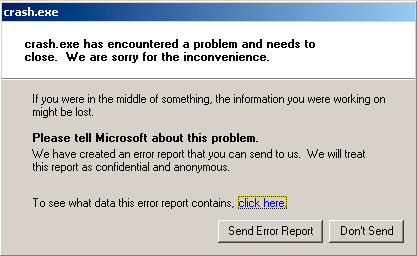
\includegraphics[width=0.6\textwidth]{OS/SEH/1/crash_xp1.png}
\caption{Windows XP}
\end{figure}

\begin{figure}[H]
\centering
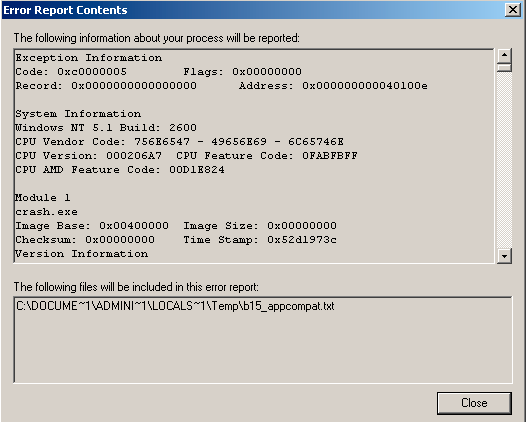
\includegraphics[width=0.6\textwidth]{OS/SEH/1/crash_xp2.png}
\caption{Windows XP}
\end{figure}

\begin{figure}[H]
\centering
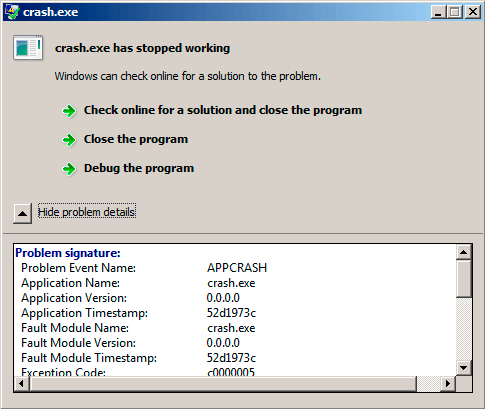
\includegraphics[width=0.6\textwidth]{OS/SEH/1/crash_win7.png}
\caption{Windows 7}
\end{figure}

\begin{figure}[H]
\centering
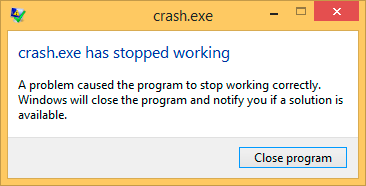
\includegraphics[width=0.6\textwidth]{OS/SEH/1/crash_win81.png}
\caption{Windows 8.1}
\end{figure}

Historiquement, cette chaîne de gestionnaires était connue sous l'appellation Dr. Watson
\footnote{\href{https://en.wikipedia.org/wiki/Dr._Watson_(debugger)}{Wikipédia}}.

Certains développeurs ont eu l'idée d'écrire leur propre gestionnaire d'exceptions pour recevoir
les informations relatives au crash.
\myindex{Windows!Win32!SetUnhandledExceptionFilter()}
Ils enregistrent leur gestionnaire en appelant la fonction \TT{SetUnhandledExceptionFilter()} qui
sera alors appelée si l'\ac{OS} ne trouve aucun autre gestionnaire qui souhaite gérer l'exception.

\myindex{\oracle}
\oracle--- en est un bon exemple qui sauvegarde un énorme fichier dump collectant toutes les
informations possibles concernant la \ac{CPU} et l'état de la mémoire.

Écrivons notre propre gestionnaire d'exception. Cet exemple s'appuie sur celui de \PietrekSEH.
Pour le compiler, il faut utiliser l'option SAFESEH : \TT{cl seh1.cpp /link /safeseh:no}.
Vous trouverez plus d'informations concernant SAFESEH à: \href{http://msdn.microsoft.com/en-us/library/9a89h429.aspx}{MSDN}.

\lstinputlisting[style=customc]{OS/SEH/1/1.cpp}

En environnement win32, le registre de segment FS: contient l'adresse du \ac{TIB}.

Le tout premier élément de la structure \ac{TIB} est un pointeur sur le premier gestionnaire de la
chaîne de traitement des exceptions.
Nous le sauvegardons sur la pile et remplaçons la valeur par celle de notre propre gestionnaire.
La structure est du type \TT{\_EXCEPTION\_REGISTRATION}. Il s'agit d'une simple liste chaînée dont
les éléments sont conservés sur la pile.

\begin{lstlisting}[caption=MSVC/VC/crt/src/exsup.inc,style=customasmx86]
_EXCEPTION_REGISTRATION struc
     prev    dd      ?
     handler dd      ?
_EXCEPTION_REGISTRATION ends
\end{lstlisting}

Le champ \q{handler} contient l'adresse du gestionnaire et le champ \q{prev} celle de
l'enregistrement suivant dans la chaîne.
Le dernier enregistrement contient la valeur \TT{0xFFFFFFFF} (-1) dans son champ \q{prev}.

\begin{center}
\begin{tikzpicture}[thick,scale=0.75, every node/.style={scale=0.75}]
	\tikzstyle{every path}=[thick]
	\tikzstyle{undefined}=[draw,rectangle,minimum height=1cm, minimum width=3.5cm, text width=3.5cm]
	\tikzstyle{node}=[draw,rectangle,minimum height=1cm, minimum width=3.5cm, text width=3.5cm, fill=gray!20]
	
	\node[node] (fs) [minimum width=1.5cm, text width=1.5cm] {FS:0};

	\node[node] (tib1) [right=1.5cm of fs] {+0: \_\_except\_list};
	\node[undefined] (tib2) [below of=tib1] {+4: \dots};
	\node[undefined] (tib3) [below of=tib2] {+8: \dots};
	\node (tib_text) [above of=tib1] {TIB};
	
	\draw [->] (fs.east) -- (tib1.west);

	\node[undefined] (u1) [text centered, right=2.5cm of tib1] {\dots};
	\node [node] (n1prev) [below of=u1] {Prev=0xFFFFFFFF};
	\node [node] (n1handler) [below of=n1prev] {Handle};
	\node [node] (n1handler_text) [right=1cm of n1handler] {\HandlerFunction};
	\draw [->] (n1handler.east) -- (n1handler_text.west);
	\node[undefined] (u2) [text centered, below of=n1handler] {\dots};
	\node [node] (n2prev) [below of=u2] {Prev};
	\node [node] (n2handler) [below of=n2prev] {Handle};
	\node [node] (n2handler_text) [right=1cm of n2handler] {\HandlerFunction};
	\draw [->] (n2handler.east) -- (n2handler_text.west);
	\node[undefined] (u3) [text centered, below of=n2handler] {\dots};
	\node [node] (n3prev) [below of=u3] {Prev};

	\node [node] (n3handler) [below of=n3prev] {Handle};
	\node [node] (n3handler_text) [right=1cm of n3handler] {\HandlerFunction};
	\draw [->] (n3handler.east) -- (n3handler_text.west);
	\node[undefined] (u4) [text centered, below of=n3handler] {\dots};
	\node (stack_text) [above of=u1] {\RU{Стек}\EN{Stack}};
	
	\node (n2block_pt1) [inner sep=0pt, above left=0cm and 0cm of n2prev] {};
	\node (n2block_pt2) [inner sep=0pt, above left=0cm and 0.5cm of n2prev] {};
	\draw [->] (n3prev.west) .. controls +(left:0.5cm) and (n2block_pt2) .. (n2block_pt1);

	\node (n1block_pt1) [inner sep=0pt, above left=0cm and 0cm of n1prev] {};
	\node (n1block_pt2) [inner sep=0pt, above left=0cm and 0.8cm of n1prev] {};
	\draw [->] (n2prev.west) .. controls +(left:0.8cm) and (n1block_pt2) .. (n1block_pt1);
	
	\node (n3block_pt1) [inner sep=0pt, above left=0cm and 0cm of n3prev] {};
	\node (n3block_pt2) [inner sep=0pt, above left=0cm and 1.25cm of n3prev] {};
	\draw [->] (tib1.east) .. controls +(right:1.25cm) and (n3block_pt2) .. (n3block_pt1);


\end{tikzpicture}
\end{center}


Une fois notre gestionnaire installé, nous invoquons la fonction \TT{RaiseException()}
\footnote{\href{http://msdn.microsoft.com/en-us/library/windows/desktop/ms680552(v=vs.85).aspx}{MSDN}}.
Il s'agit d'une exception utilisateur.
Le gestionnaire vérifie le code.
Si le code est égal à \TT{0xE1223344}, il retourne la valeur \TT{ExceptionContinueExecution} qui
signifie que le gestionnaire a corrigé le contenu de la structure passée en paramètre qui décrit
l'état de la CPU. La modification concerne généralement les registres EIP/ESP. L'\ac{OS} peut alors
reprendre l'exécution du thread.

Si vous modifiez légèrement le code pour que le gestionnaire retourne la valeur \TT{ExceptionContinueSearch},
l'\ac{OS} appellera les gestionnaires suivants dans la liste. Il est peu probable que l'un d'eux sache
la gérer puisqu'aucun d'eux ne la comprend, ni ne connaît le code exception.
Vous verrez donc apparaître la boîte de dialogue Windows précurseur du crash.

Quelles sont les différences entre les exceptions système et les exceptions utilisateur ?
Les exceptions système sont listées ci-dessous:

\small
\begin{center}
\begin{tabular}{ | l | l | l | }
\hline
\HeaderColor as defined in WinBase.h &
\HeaderColor as defined in ntstatus.h &
\HeaderColor value \\
\hline
EXCEPTION\_ACCESS\_VIOLATION          & STATUS\_ACCESS\_VIOLATION           & 0xC0000005 \\
\hline
EXCEPTION\_DATATYPE\_MISALIGNMENT     & STATUS\_DATATYPE\_MISALIGNMENT      & 0x80000002 \\
\hline
EXCEPTION\_BREAKPOINT                & STATUS\_BREAKPOINT                 & 0x80000003 \\
\hline
EXCEPTION\_SINGLE\_STEP               & STATUS\_SINGLE\_STEP                & 0x80000004 \\
\hline
EXCEPTION\_ARRAY\_BOUNDS\_EXCEEDED     & STATUS\_ARRAY\_BOUNDS\_EXCEEDED      & 0xC000008C \\
\hline
EXCEPTION\_FLT\_DENORMAL\_OPERAND      & STATUS\_FLOAT\_DENORMAL\_OPERAND     & 0xC000008D \\
\hline
EXCEPTION\_FLT\_DIVIDE\_BY\_ZERO        & STATUS\_FLOAT\_DIVIDE\_BY\_ZERO       & 0xC000008E \\
\hline
EXCEPTION\_FLT\_INEXACT\_RESULT        & STATUS\_FLOAT\_INEXACT\_RESULT       & 0xC000008F \\
\hline
EXCEPTION\_FLT\_INVALID\_OPERATION     & STATUS\_FLOAT\_INVALID\_OPERATION    & 0xC0000090 \\
\hline
EXCEPTION\_FLT\_OVERFLOW              & STATUS\_FLOAT\_OVERFLOW             & 0xC0000091 \\
\hline
EXCEPTION\_FLT\_STACK\_CHECK           & STATUS\_FLOAT\_STACK\_CHECK          & 0xC0000092 \\
\hline
EXCEPTION\_FLT\_UNDERFLOW             & STATUS\_FLOAT\_UNDERFLOW            & 0xC0000093 \\
\hline
EXCEPTION\_INT\_DIVIDE\_BY\_ZERO        & STATUS\_INTEGER\_DIVIDE\_BY\_ZERO     & 0xC0000094 \\
\hline
EXCEPTION\_INT\_OVERFLOW              & STATUS\_INTEGER\_OVERFLOW           & 0xC0000095 \\
\hline
EXCEPTION\_PRIV\_INSTRUCTION          & STATUS\_PRIVILEGED\_INSTRUCTION     & 0xC0000096 \\
\hline
EXCEPTION\_IN\_PAGE\_ERROR             & STATUS\_IN\_PAGE\_ERROR              & 0xC0000006 \\
\hline
EXCEPTION\_ILLEGAL\_INSTRUCTION       & STATUS\_ILLEGAL\_INSTRUCTION        & 0xC000001D \\
\hline
EXCEPTION\_NONCONTINUABLE\_EXCEPTION  & STATUS\_NONCONTINUABLE\_EXCEPTION   & 0xC0000025 \\
\hline
EXCEPTION\_STACK\_OVERFLOW            & STATUS\_STACK\_OVERFLOW             & 0xC00000FD \\
\hline
EXCEPTION\_INVALID\_DISPOSITION       & STATUS\_INVALID\_DISPOSITION        & 0xC0000026 \\
\hline
EXCEPTION\_GUARD\_PAGE                & STATUS\_GUARD\_PAGE\_VIOLATION       & 0x80000001 \\
\hline
EXCEPTION\_INVALID\_HANDLE            & STATUS\_INVALID\_HANDLE             & 0xC0000008 \\
\hline
EXCEPTION\_POSSIBLE\_DEADLOCK         & STATUS\_POSSIBLE\_DEADLOCK          & 0xC0000194 \\
\hline
CONTROL\_C\_EXIT                      & STATUS\_CONTROL\_C\_EXIT             & 0xC000013A \\
\hline
\end{tabular}
\end{center}
\normalsize

Le code de chaque exception se décompose comme suit:

\begin{center}
\begin{bytefield}[bitwidth=0.03\linewidth]{32}
\bitheader[endianness=big]{31,29,28,27,16,15,0} \\
\bitbox{2}{S} &
\bitbox{1}{U} &
\bitbox{1}{0} &
\bitbox{12}{Facility code} &
\bitbox{16}{Error code}
\end{bytefield}
\end{center}

S est un code status de base:
11---erreur;
10---warning;
01---information;
00---succès.
U---lorsqu'il s'agit d'un code utilisateur.

Voici pourquoi nous choisissons le code 0xE1223344---E\textsubscript{16} (1110\textsubscript{2}) 0xE (1110b)
qui signifie 1) qu'il s'agit d'une exception utilisateur; 2) qu'il s'agit d'une erreur.

Pour être honnête, l'exemple fonctionne aussi bien sans ces bits de poids fort.

Tentons maintenant de lire la valeur à l'adresse mémoire 0.

Bien entendu, dans win32 il n'existe rien à cette adresse, ce qui déclenche une exception.

Le premier gestionnaire à être invoqué est le vôtre. Il reconnaît l'exception car il compare
le code avec celui de la constante \TT{EXCEPTION\_ACCESS\_VIOLATION}.

Le code qui lit la mémoire à l'adresse 0 ressemble à ceci:

\lstinputlisting[style=customasmx86,caption=MSVC 2010]{OS/SEH/1/1_fragment.asm}

Serait-il possible de corriger cette erreur \q{au vol} afin de continuer l'exécution du programme?

Notre gestionnaire d'exception peut modifier la valeur du registre \EAX puis laisser l'\ac{OS}
exécuter de nouveau l'instruction fautive.
C'est ce que nous faisons et la raison pour laquelle \printf affiche 1234. Lorsque notre gestionnaire
a fini son travail, la valeur de \EAX n'est plus 0 mais l'adresse de la variable globale \TT{new\_value}.
L'exécution du programme se poursuit donc.

Voici ce qui se passe: le gestionnaire mémoire de la \ac{CPU} signale une erreur, la \ac{CPU} suspend
le thread, trouve le gestionnaire d'exception dans le noyau Windows, lequel à son tour appelle les
gestionnaires de la chaîne \ac{SEH} un par un.

Nous utilisons ici le compilateur MSVC 2010. Bien entendu, il n'y a aucune garantie que celui-ci
décide d'utiliser le registre \EAX pour conserver la valeur du pointeur.

Le truc du remplacement du contenu du registre n'est qu'une illustration de ce que peut être le
fonctionnement interne des \ac{SEH}.
En pratique, il est très rare qu'il soit utilisé pour corriger \q{on-the-fly} une erreur.

Pourquoi les enregistrements SEH sont-ils conservés directement sur la pile et non pas à un autre
endroit?

L'explication la plus plausible est que l'\ac{OS} n'a ainsi pas besoin de libérer l'espace qu'ils
utilisent. Ces enregistrements sont automatiquement supprimés lorsque la fonction se termine.
\myindex{\CStandardLibrary!alloca()}
C'est un peu comme la fonction alloca(): (\myref{alloca}).

